% !TEX encoding = UTF-8
% !TEX program = pdflatex
% !TEX root = InformationRetrieval.tex
% !TEX spellcheck = it-IT

% 16 Dicembre 2016

\subsection{Assessment con ANOVA - Validazione del modello}

Dato un gruppo con diversi fattori cerca di determinare se le medie sono uguali oppure no.

Ad esempio ho 3 farmaci da dare a devi vari pazienti e devo capire se i farmaci hanno effetti diversi, assumendo che l'effetto dei farmaci posso essere modellato con delle distribuzioni gaussiane.
Ci sia aspetta che se i farmaci hanno effetti diversi i valori medi sperimentali siano diversi. 
La tecnica ANOVA serve per capire se effettivamente è ragionevole assumere che anche la media reale sia diversa, oppure che le medie siano diverse per via del particolare campionamento.

Più formalmente il metodo si basa sull'ipotesi nulla, che tutte le medie siano uguali. Ovvero tutti i farmaci hanno lo stesso effetto o nel contesto dell'IR, tutti i sistemi di IR sono uguali.
La verifica dell'ipotesi viene effettuata utilizzando la $t$-di Student.

Si ha poi che il metodo ANOVA ragiona sulla varianza totale del modello, scomponendola negli effetti delle singole componenti.
Pertanto questo metodo può essere applicato anche per modelli più complessi che prendono in considerazione i vari componenti di un sistema IR, infatti, al variare dei componenti possiamo osservare come varia la varianza delle prestazioni del sistema e, se un componente del sistema è significativo l'utilizzarlo o meno porta ad una variazione della media.

Dal lato statistico questo funziona perché la verifica dell'ipotesi $H_0$ viene fatta considerando le variane, le quali si comportano in un certo modo se le medie sono uguali e in un altro se sono diverse.

La scomposizione della varianza parte dalla formulazione del nostro modello:

\begin{align*}
Y_{ij} &= \underbrace{\hat{\mu}_{\cdot \cdot} + \hat{\tau_i} + \hat{\alpha}_j}_{Modello} + \underbrace{\hat{\epsilon}_{ij}}_{Errore} \\
\underbrace{Y_{ij} - \hat{\mu}_{\cdot \cdot}}_{\text{Effetto totale}} &= \underbrace{\hat{\mu}_{i\cdot} - \hat{\mu}_{\cdot \cdot}}_{\text{Effetto del soggeto}}  + \underbrace{\hat{\mu}_{\cdot j} - \hat{\mu}_{\cdot \cdot}}_{\text{Effetto del fattore}} + \underbrace{T_{ij} - (\hat{\mu}_{i \cdot }+ \hat{\mu}_{\cdot j} - \hat{\mu}_{\cdot \cdot}  )}_{\text{Effetto degli errori}}
\end{align*}

Le singole varianze vengono quindi calcolate prendendo la somma degli scarti quadrati e dei gradi di libertà di ogni componente.

\begin{align*}
SS_{tot} &= \sum\limits_{j=1}^{p}\sum\limits{i=1}^{n} (Y_{ij} - \hat{\mu}_{\cdot\cdot})^2 \\
SS_{sogg} &= \sum\limits_{j=1}^{p}\sum\limits{i=1}^{n} (\hat{\mu}_{i\cdot} - \hat{\mu}_{\cdot\cdot})^2 = \sum\limits{i=1}^{n} p(\hat{\mu}_{i\cdot} - \hat{\mu}_{\cdot\cdot})^2 \\
SS_{fatt} &= \sum\limits_{j=1}^{p}\sum\limits{i=1}^{n} (\hat{\mu}_{\cdot j} - \hat{\mu}_{\cdot\cdot})^2 = \sum\limits{j=1}^{p} n(\hat{\mu}_{\cdot j} - \hat{\mu}_{\cdot\cdot})^2 \\
SS_{tot} &= \sum\limits_{j=1}^{p}\sum\limits{i=1}^{n} (Y_{ij} - (\hat{\mu}_{i \cdot }+ \hat{\mu}_{\cdot j} - \hat{\mu}_{\cdot \cdot}  ))^2
\end{align*}

La stima della varianza viene quindi fatta dividendo le varie somme per i loro gradi di libertà.

\begin{align*}
MS_{tot} &= \frac{SS_{tot}}{df_{tot}} = \frac{SS_{tot}}{pn-1}\\
MS_{sogg} &= \frac{SS_{sogg}}{df_{sogg}} = \frac{SS_{sogg}}{n-1}\\
MS_{fatt} &= \frac{SS_{fatt}}{df_{fatt}} = \frac{SS_{fatt}}{p-1}\\
MS_{err} &= \frac{SS_{err}}{df_{err}} = \frac{SS_{err}}{(n-1)(p-1)}
\end{align*}

Il test sull'ipotesi $H_0$ viene fatto utilizzando queste stime, perché se le medie sono tutte uguali, ovvero non c'è differenza tra i sistemi, il rapporto tra la varianza stimata di un componente e quella degli errori segue la distribuzione $F_{df_{fatt}, df_{err}}$.

Viene quindi calcolato un valore $F_{fatt}$ che più grande risulta, minore è la probabilità che $H_0$ sia vera.

$$
F_{fatt} = \frac{MS_{fatt}}{MS_{err}}
$$

Il valore così ottenuto viene controllato con un test sul livello di significatività $\alpha$.

Si deve quindi prima fissare un valore per $\alpha$, per poi trovare il corrispettivo valore $F_{crit}$ della distribuzione $F$ tale che l'area della curva a destra di $F_{crit}$ sia pari ad $\alpha$. Se $F_{fatt} > F_{crit}$, ovvero il p-value\footnote{Il $p$-value è la probabilità di ottenere un altro dato più estremo di quello osservato $F_{fatt}$, ovvero l'area della curva a destra di $F_{fatt}$ nella distribuzione di riferimento.} allora è possibile assumere che $H_0$ sia falsa con significatività $1 - \alpha$. 

\begin{figure}[htbp]
	\centering
	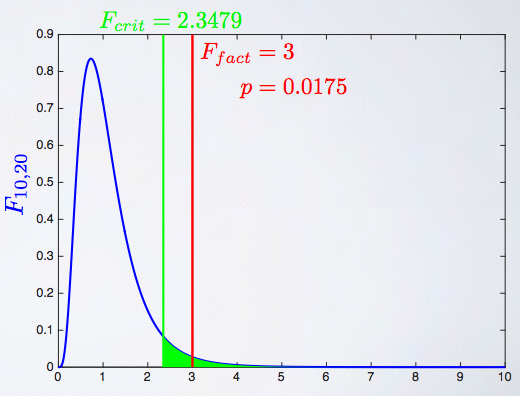
\includegraphics[width=0.6\textwidth]{images/l21-fig-1}
	\caption{Esempio di test di significatività sull'ipotesi $H_0$.}
\end{figure}

Il tutto può essere riassunto in una tabella ANOVA, che riporta i vari risultati delle somme.

Ad esempio, per l'heatmap precedente e considerando il modello fin'ora utilizzato (topic e sistema), la tabella ANOVA è la seguente.

\begin{table}[htbp]
	\centering
	\begin{tabular}{|c|c|c|c|c|c|}
		\hline
		\textbf{Source}  & \textbf{SS} & \textbf{DF} & \textbf{MS} & \textbf{F} & \textbf{p-value} \\ \hline
		\textbf{Topics}  & 820.99      & 49          & 16.75       & 694.7235   & 0                \\ \hline
		\textbf{Systems} & 36.44       & 399         & 0.09        & 7.4464     & 0                \\ \hline
		\textbf{Error}   & 88.20       & 19551       & 0.0049      &            &                  \\ \hline
		\textbf{Total}   & 945.63      & 19999       &             &            &                  \\ \hline
	\end{tabular}
	\caption{Tabella ANOVA per il modello Topic-Sistema}\label{my-label}
\end{table}

Dalla tabella si può notare che i topics influenzano la maggior parte della varianza totale con significatività molto alta\footnote{$p$-value uguale a 0.}, ma in ogni caso l'effetto dei sistemi è statisticamente significativo per la varianza e quindi tutto il lavoro legato all'information retrieval ha senso.

Facendo varie prove si è osservato che quanto riportato non vale solo per il caso specifico della heatmap precedente (AP su TREC08) ma è valido anche per altre collezioni e misure.
Si è inoltre osservato che al variare della misura utilizzata (nDCG@20, AP, ecc.) varia anche l'effetto del sistema, che risulta maggiore in caso di nDCG@20.

\section{Grid of Points}

Lo stesso ragionamento utilizzato per il modello a singolo fattore è stato applicato più nel dettaglio prendendo in considerazione anche l'effetto delle stop list, dello stemmer e del modello di reperimento.

Ognuna di queste combinazioni (560) sono state provate con Terrier su varie collezioni e sono state raccolte varie misure.

Il modello a singolo fattore è stato quindi esteso ad un modello a tre fattori, dove il contributo del sistema $\alpha_j$ viene spezzato nell'effetto della stop list, dello stemmer e del modello, tenendo in considerazione anche le coppie degli effetti:

$$
Y_{ijkl} = \mu_{\cdot\cdot\cdot\cdot} + \tau_i + \alpha_j + \beta_k + \gamma_l + \alpha\beta_{jk} + \alpha\gamma_{jl} + \beta\gamma_{kl}+\alpha\beta\gamma{jkl} + \epsilon_{ijkl}
$$

Tutti i conti precedenti possono essere adottati, solo che anziché essere applicati su una matrice vengono applicati su un cubo a 4 dimensioni.

Dalla tabella ANOVA (tabella \ref{tab:anova-3}) risultate per l'average precision su TREC08 si può notare che solamente gli effetti di primo ordine sono significativi, mentre quelli combinati non spiegano molta varianza.
In termini pratici questo ci va bene perché vuol dire che la varianza dipende dai singoli componenti e non da come questi interagiscono tra loro.
Sempre dalla tabella si può notare che la maggior parte della varianza spiegata dal sistema è spiegata dalla stop list, il che è stato un risultato inaspettato perché si credeva che la stop list venisse utilizzata solamente per una questione di efficienza/riduzione dei dati e non tanto per scartare le parole ad alta frequenza, perché dovrebbe essere in grado il modello di gestirle ed inoltre la frequenza delle parole è influenzata dal dominio della collezione.

\begin{table}[htbp]
	\centering
	\begin{tabular}{|l|c|c|c|c|c|}
		\hline
		\multicolumn{1}{|c|}{\textbf{Source}} & \textbf{SS} & \textbf{DF} & \textbf{MS} & \textbf{F} & \textbf{p} \\ \hline
		\textbf{Topics}                       & 820.99      & 49          & 16.75       & 3713.90    & 0.00       \\ \hline
		\textbf{Stop list}                    & 9.89        & 4           & 2.47        & 548.06     & 0.00       \\ \hline
		\textbf{Stemmer}                      & 4.16        & 4           & 1.04        & 230.76     & 0.00       \\ \hline
		\textbf{Model}                        & 5.16        & 15          & 0.3443      & 76.32      & 0.00       \\ \hline
		\textbf{Stop list*Stemmer}            & 0.05        & 16          & 0.03        & 0.67       & 0.83       \\ \hline
		\textbf{Stop list*Model}              & 17.01       & 60          & 0.28        & 62.84      & 0.00       \\ \hline
		\textbf{Stemmer*Model}                & 0.07        & 60          & 0.001       & 0.26       & 1.00       \\ \hline
		\textbf{Stop list*Stemmer*Model}      & 0.09        & 240         & 0.00        & 0.08       & 1.00       \\ \hline
		\textbf{Error}                        & 88.20       & 19551       & 0.005       &            &            \\ \hline
		\textbf{Total}                        & 945.63      & 19999       &             &            &            \\ \hline
	\end{tabular}
	\caption{Tabella ANOVA per il modello a tre fattori.}\label{tab:anova-3}
\end{table}

\subsection{Guardando avanti}

La stesso sistema di valutazione può essere ulteriormente esteso prendendo in considerazione anche l'effetto della lingua.
Però così nascono ulteriori problemi, riguardo l'utilizzo di stemmer e modelli in grado di funzionare con più lingue e anche riguardo i topic, perché servono collezioni in lingua diversa ma con gli stessi topic per le varie lingue.
Ci sono poi anche i problemi più pratici come la codifica del file e la tokenzzazione.


In ogni caso l'importante è capire come è possibile utilizzare questo sistema per avere un riferimento in modo da riuscire a capire se si sta migliorando o meno e magari in un secondo momento essere in grado di sfruttare questo sistema di valutazione per predire le prestazioni di un sistema IR prima di implementarlo. 
Tenendo sempre a mente che le misure così ottenute non hanno un valore assoluto, perché basta anche un piccolo cambiamento in una stop list per far variare i valori.






